\chapter{Optický přenost dat}
\zkratka{LG} je založeno na optickém přenosu dat ze zbraně do vesty. Tato data jsou naprosto klíčová, nesou v sobě informace o tom, kdo je vyslal a chyba při přenosu nebo interpretaci těchto dat, by byla fatální. V nejhorším případě by mohla způsobit přičtení bodů špatnému hráči, což by poškodilo střelce a při kumulaci těchto chyb by \zkratka{LG} hráče brzy omrzela. Proto je potřeba se problematikou optického přenosu dat zabývat.

Při \zkratka{LG} jsou data přenášena v infračerveném pásmu elektromagnetických vln, což odpovídá vlnovým délkám $\lambda \in \langle 760~\jedn{nm};~1~\jedn{mm}\rangle$. Tyto vlnové délky jsou pro lidské oko nedetekovalné a tak si běžný hráč přenášených dat, ani nevšimne.

\subsection{Optické vysílače}
Optické vysílače obdobně jako vysílače rádiové slouží k vysílání elektromagnetických vln. Od rádiových vysílačů  se odlišují tím, že využívají jinou část elektromagnetického spektra $\lambda \in \langle 10~\jedn{nm}~;~1~\jedn{mm}  \rangle$, tedy od infračerveného záření, přes viditelné světlo až po záření ultra fialové. Vysílače můžeme rozdělit do dvou skupin a to vysílače založené na \zkratka{LED} a na laseru.

\subsubsection{LED}
Luminiscenční diody jsou polovodičové součástky s jedním PN přechodem. Na rozdíl od klasických diod nemají \zkratka{LED} obě vrstvy PN přechodu stejně dotované. Polovodič N je mnohem více dotován, navíc má mnohem větší objem než polovodič P. Díky tomu, pokud diodou prochází proud, tak převažuje přesun nosičů z oblasti N do oblasti P, kde rekombinují a uvolněná energie je přeměněna na světelné záření a tepelnou energii. Vrstva P je tenká, aby nedocházelo k velkým ztrátám, při šíření světla z polovodiče do okolního prostředí. Vlnová délka vyzařovaného světla je dána použitým základním materiálem. Pokud známe vlnovou délku, můžeme si spočítat potřebou energii, kterou je třeba elektronům udělit, aby \zkratka{LED} svítila.

$$ E = hf = \dfrac{hc}{\lambda} $$

\begin{figure}[H]
    \begin{center}
        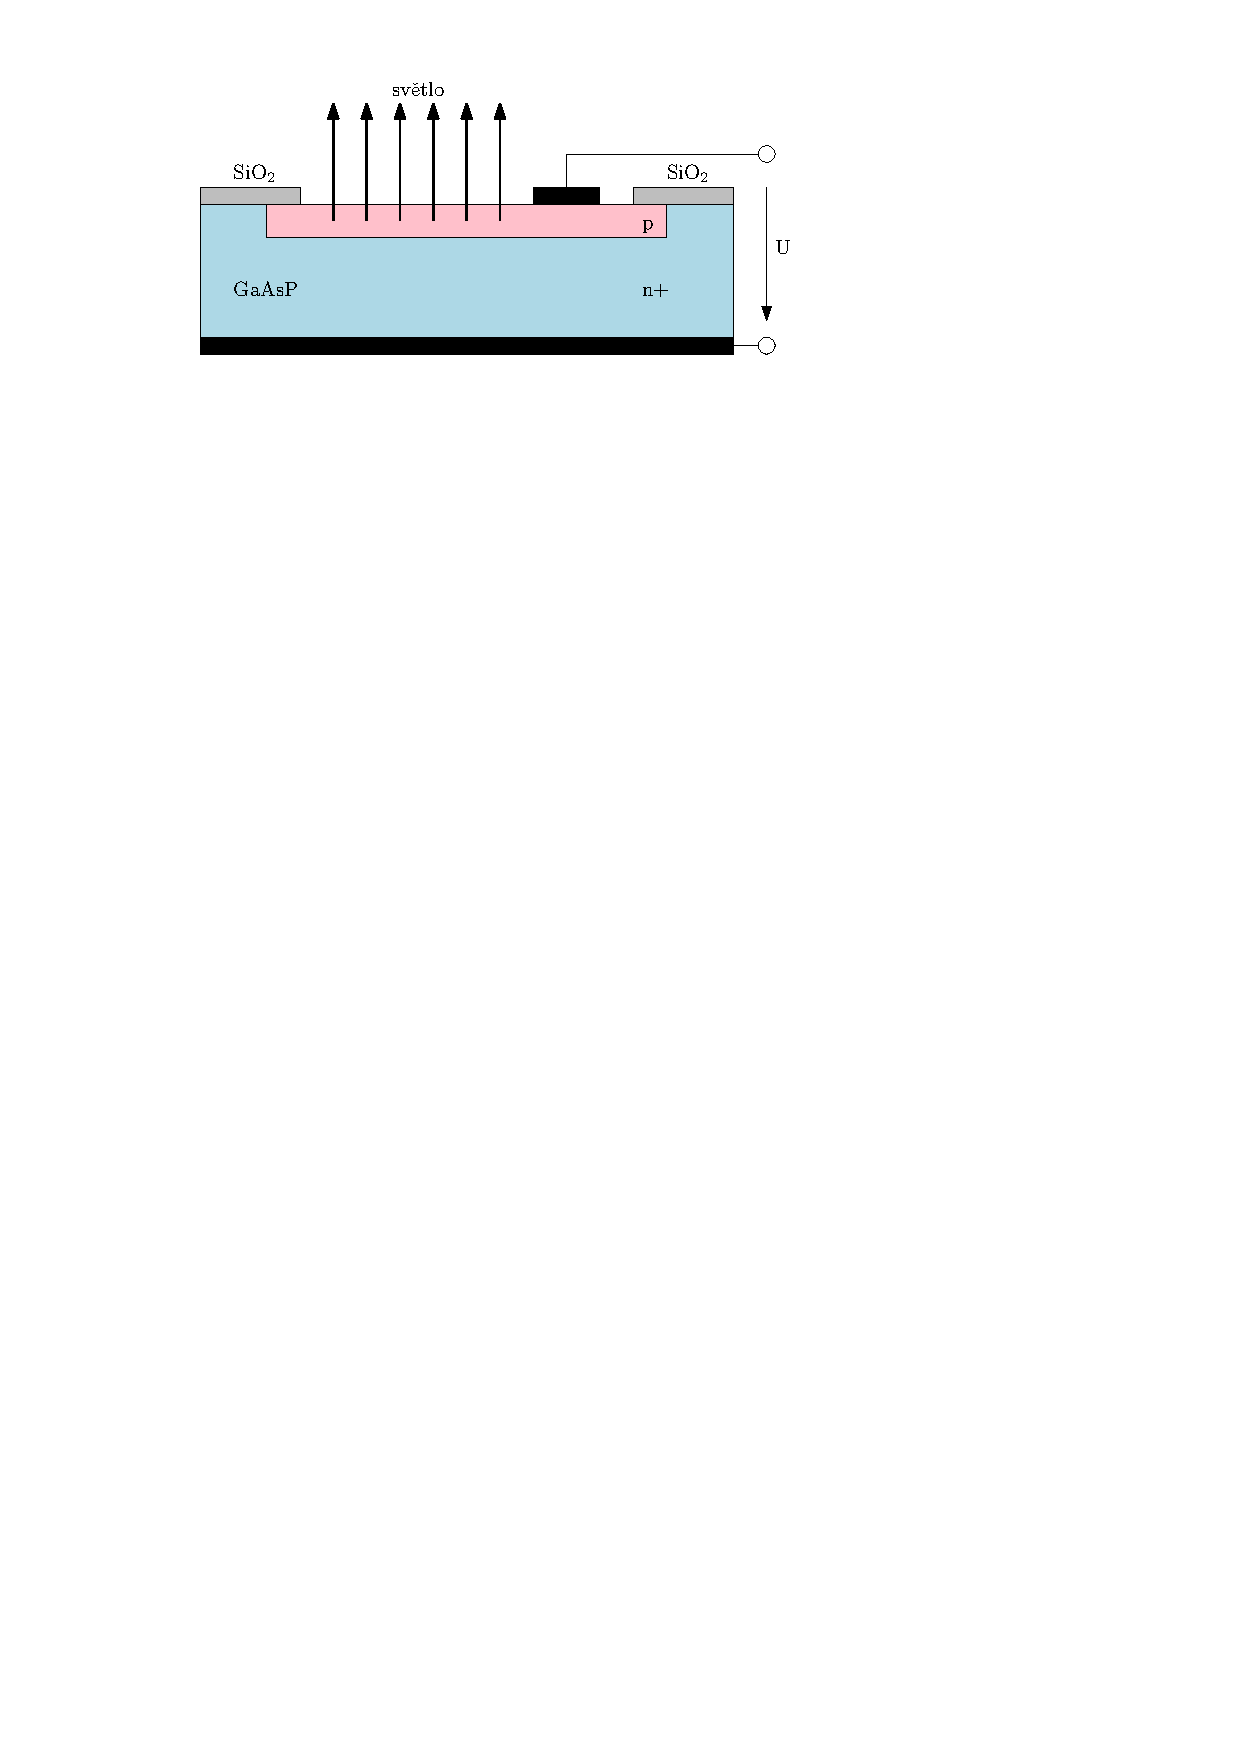
\includegraphics[scale=1]{img/led}
    \end{center}
    \caption{Technologické provedení LED pro viditelné světlo}
\end{figure}

\begin{figure}[H]
    \begin{center}
        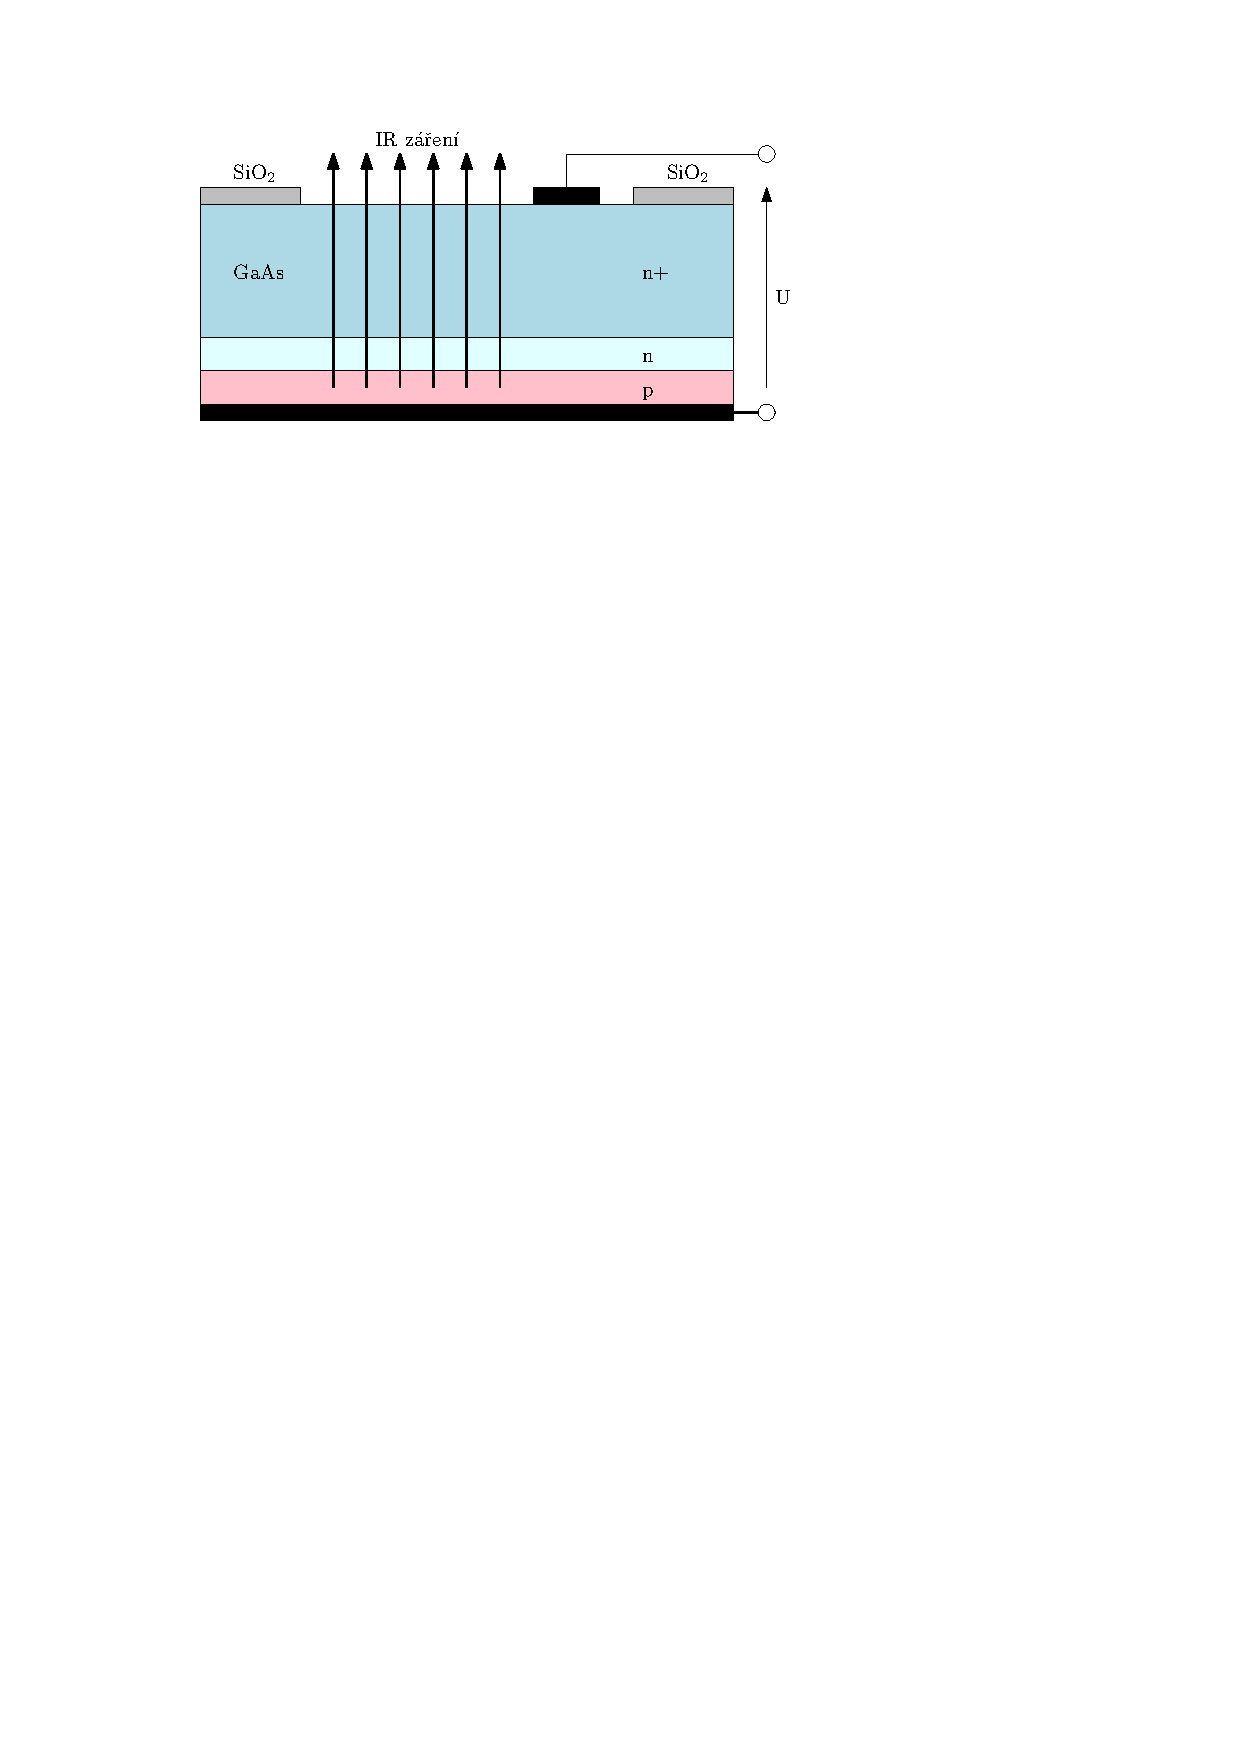
\includegraphics[scale=1]{img/ir-led}
    \end{center}
    \caption{Technologické provedení IR LED}
\end{figure}

\zkratka{IR} \zkratka{LED} jsou konstrukčně řešeny jinak. Využívá se toho, že \zkratka{IR} záření není polovodičem tlumeno tolik jako viditelné světlo. Díky tomu mohla být oblast vzniku záření umístěna do spodní části substrátu. To má velkou výhodu, protože se může snáze odvádět teplo vznikající při rekombinaci. Díky tomu mohou \zkratka{IR} \zkratka{LED} vyzařovat mnohem větší výkon než diody vyzařující viditelné světlo. Proto nalézají uplatnění jako optické vysílače, zejména na delší vzdálenosti. Základním materiálem pro výrobu \zkratka{IR} \zkratka{LED} je galiumarsenit. Vyráběné diody dosahují vlnových délek $\lambda \in \langle 830~\jedn{nm}~;~1040~\jedn{nm} \rangle$.

\subsubsection{Laserové diody}
Lasererová dioda je polovodičová součástka, která při malém proudu v propustném směru se chová jako klasická luminiscenční dioda. Proud způsobí spontánní emisi\footnote{k emisi dochází náhodně, v libovolný čas} a dioda vyzařuje světlelné záření. Při zvýšení proudu diodou přechází dioda do laserového režimu. V tomto režimu je vyzařované světlo koherentní\footnote{to znamená, že světlo má konstantní frekvenci a fázi}. To nastane díky optické rezonanci v polovodičovém krystalu a následné vynucené emisi.

\begin{figure}[H]
    \begin{center}
        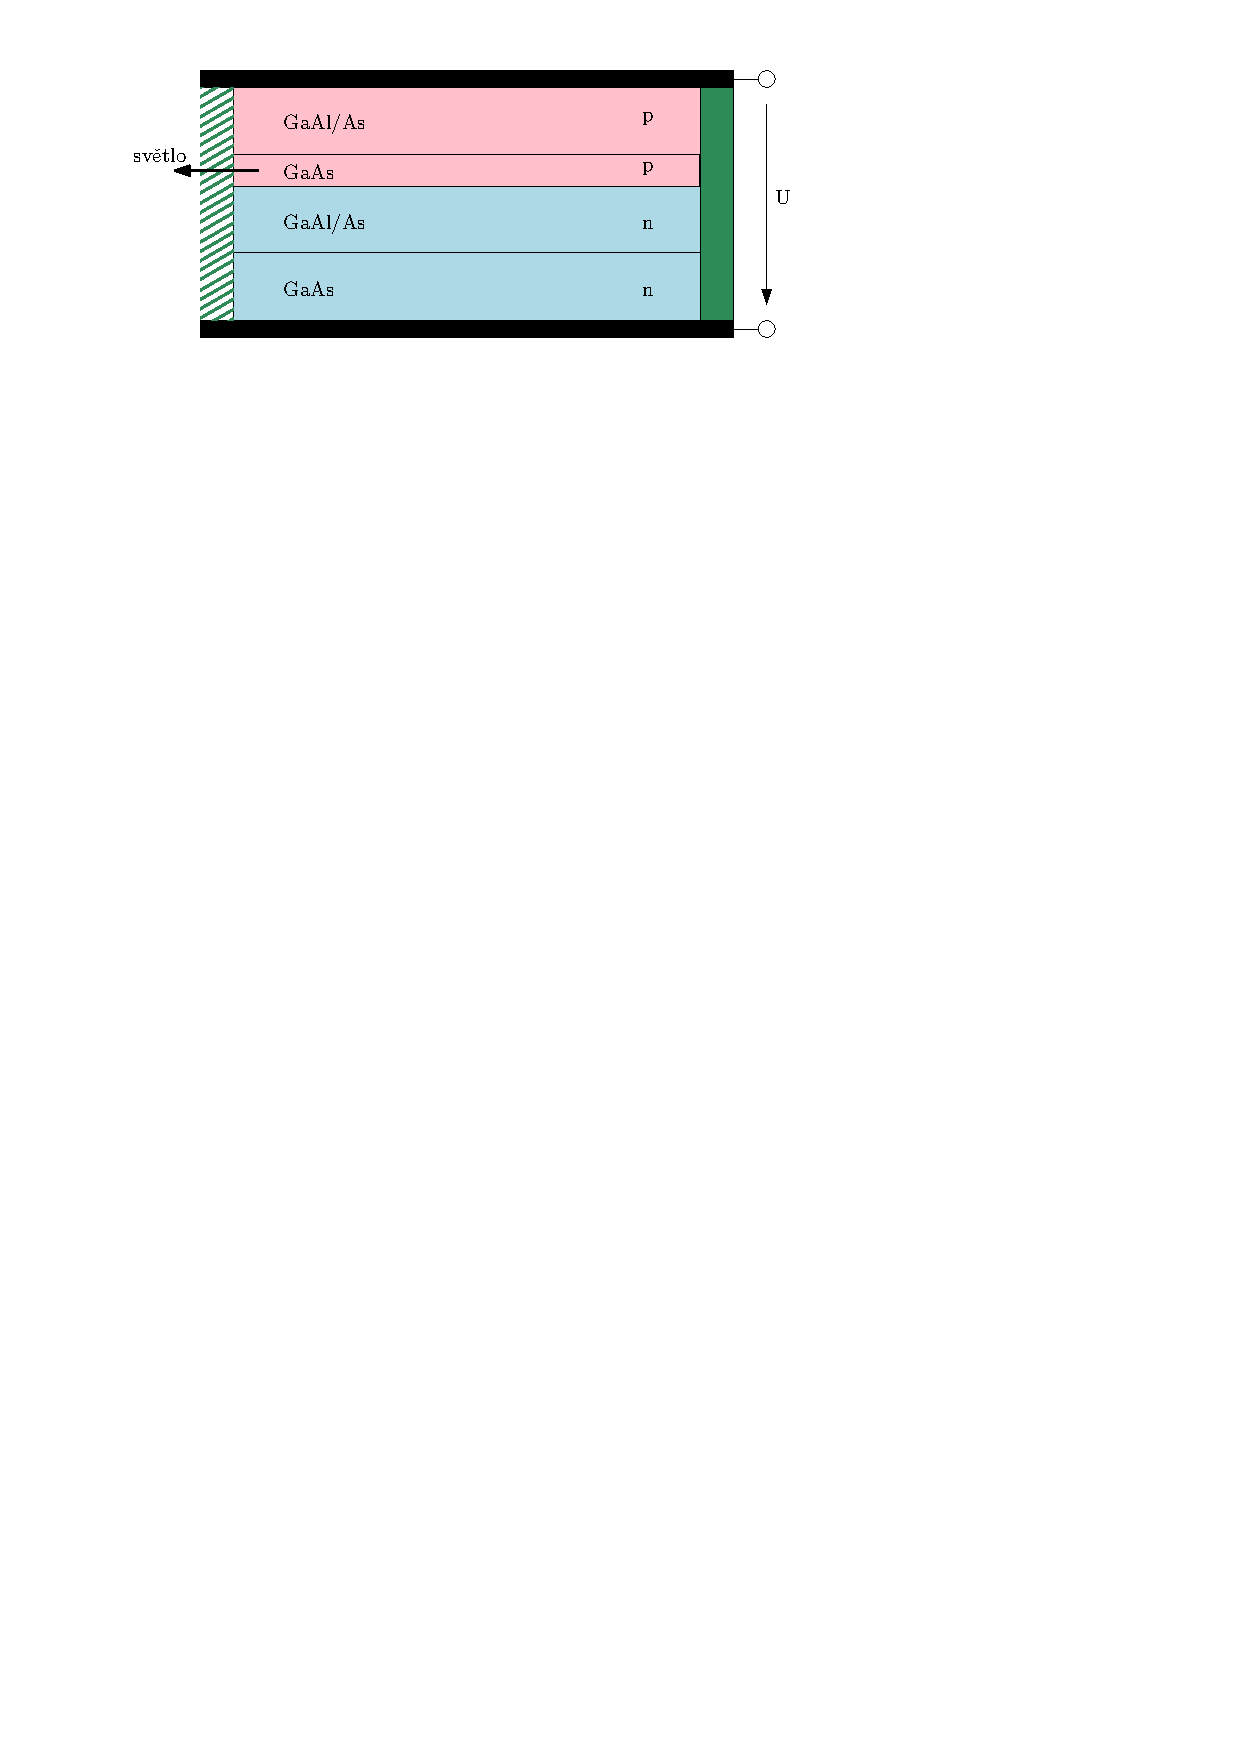
\includegraphics[scale=1]{img/laser}
    \end{center}
    \caption{Dvojitá heterogenní struktura polovodičového laseru}
\end{figure}

Emitované fotony se odráží od zrcadla a polopropustného zrcadla.  Krystal se chová jako dutinový rezonátor. Šířka a výška přechodu udává vid vznikajícího stojatého vlnění. Když překročí intenzita vlnění určitou mez, je vyzářena skrz polopropustné zrcadlo do okolí.

Laserové diody nalézají uplatnění tam, kde je třeba vyzářit velký optický výkon. Vzhledem k tomu, že v laserovém režimu se diody nachází až od vyššího proudu, tak vyžadují dobré chlazení, aby nedošlo k jejich poškození.

\subsection{Optické přijímače}
Optický přijímač nebo-li detektor či čidlo je elektrotechnická součástka, která převádí elektromagnetické vlnění o frekvencích $f \in \langle 300~\jedn{GHz}~;~100~\jedn{PHz} \rangle$ na elektrickou veličinu, nejčastěji napětí nebo proud.

\subsubsection{LED jako přijímač}
Nejjednodušším optickým přijímačem může být \zkratka{LED} dioda. Máme-li dvě totožné luminiscenční diody a jednu použijeme jako zdroj, tak pokud jí budeme svítit na druhou diodu, budeme moci mezi její anodou a katodou změřit prahové napětí.

Tento jev je způsoben tím, že dopadne-li na oblast PN přechodu foton, který má dostatečnou energii, uvolní z depletiční oblasti jeden pár díra elektron. Pokud není k diodě přiloženo vnější napětí, je v depletiční oblasti difuzní napětí. Díky difuznímu napětí je elektron urychlen do oblasti N a díra do oblasti P, tím vzniká driftový proud (proud v závěrném směru). Tento proces je označován jako fotoelektrický jev.

Pokud dopadne foton mimo vyprázdněnou oblast PN přechodu, udělí elektronu energii, díky ní, se elektron uvolní z valenční vrstvy a stane se volným nosičem náboje. Teprve poté co se elektron dostane do dopletiční oblasti, může být urychlen difuzním napětím a tím vznikne difuzní proud. Tento děj je mnohem pomalejší, než pokud foton dopadne přímo do depletiční oblasti.

\subsubsection{Fotodioda}
Fotodioda je polovodičová součástka, která je navržená pro detekování záření. Převádí dopadající elektromagnetické vlny na elektrocký proud. Konstrukčně se podobá \zkratka{LED}. Fotodiody se mohou rozdělit na dvě skupiny a to na PN fotodiody a PIN fotodiody.

PN diody nemají moc velkou oblast prostorového náboje, většina záření dopadá mimo oblast prostorového náboje. A elektronům trvá déle, než se dostanou do oblasti prostorového náboje, který je urychlí, aby vytvořili elektrocký proud. Díky tomu nejsou vhodné pro detekci rychlých signálů, ale jejich výhodou je díky jejich nízké citlivosti nízká šumovost.

PIN diody jsou oproti PN diodám mnohem rychlejší mají velkou oblast prostorového náboje a témeř všechny dopadající fotony s dostatečnou energií, uvolní elektron, který je urychlen difuzním napětím a vytvoří záporný driftový proud. Od PN diod se liší tím, že mezi vrstvou N a P mají vrstvu čistého polovodiče s vlastní vodivostí označovanou jako I. Tato vrstva se neuplatňuje při průchodu stejnosměrného proudu, dioda se chová jako běžná PN dioda. Při vyšších frekvencích nosiče náboje s vrstvy I nestihnou být odsáty. Díky tomu má vrstva I lineární odpor daný protékajícím stejnosměrným proudem.

\begin{figure}[H]
    \begin{center}
        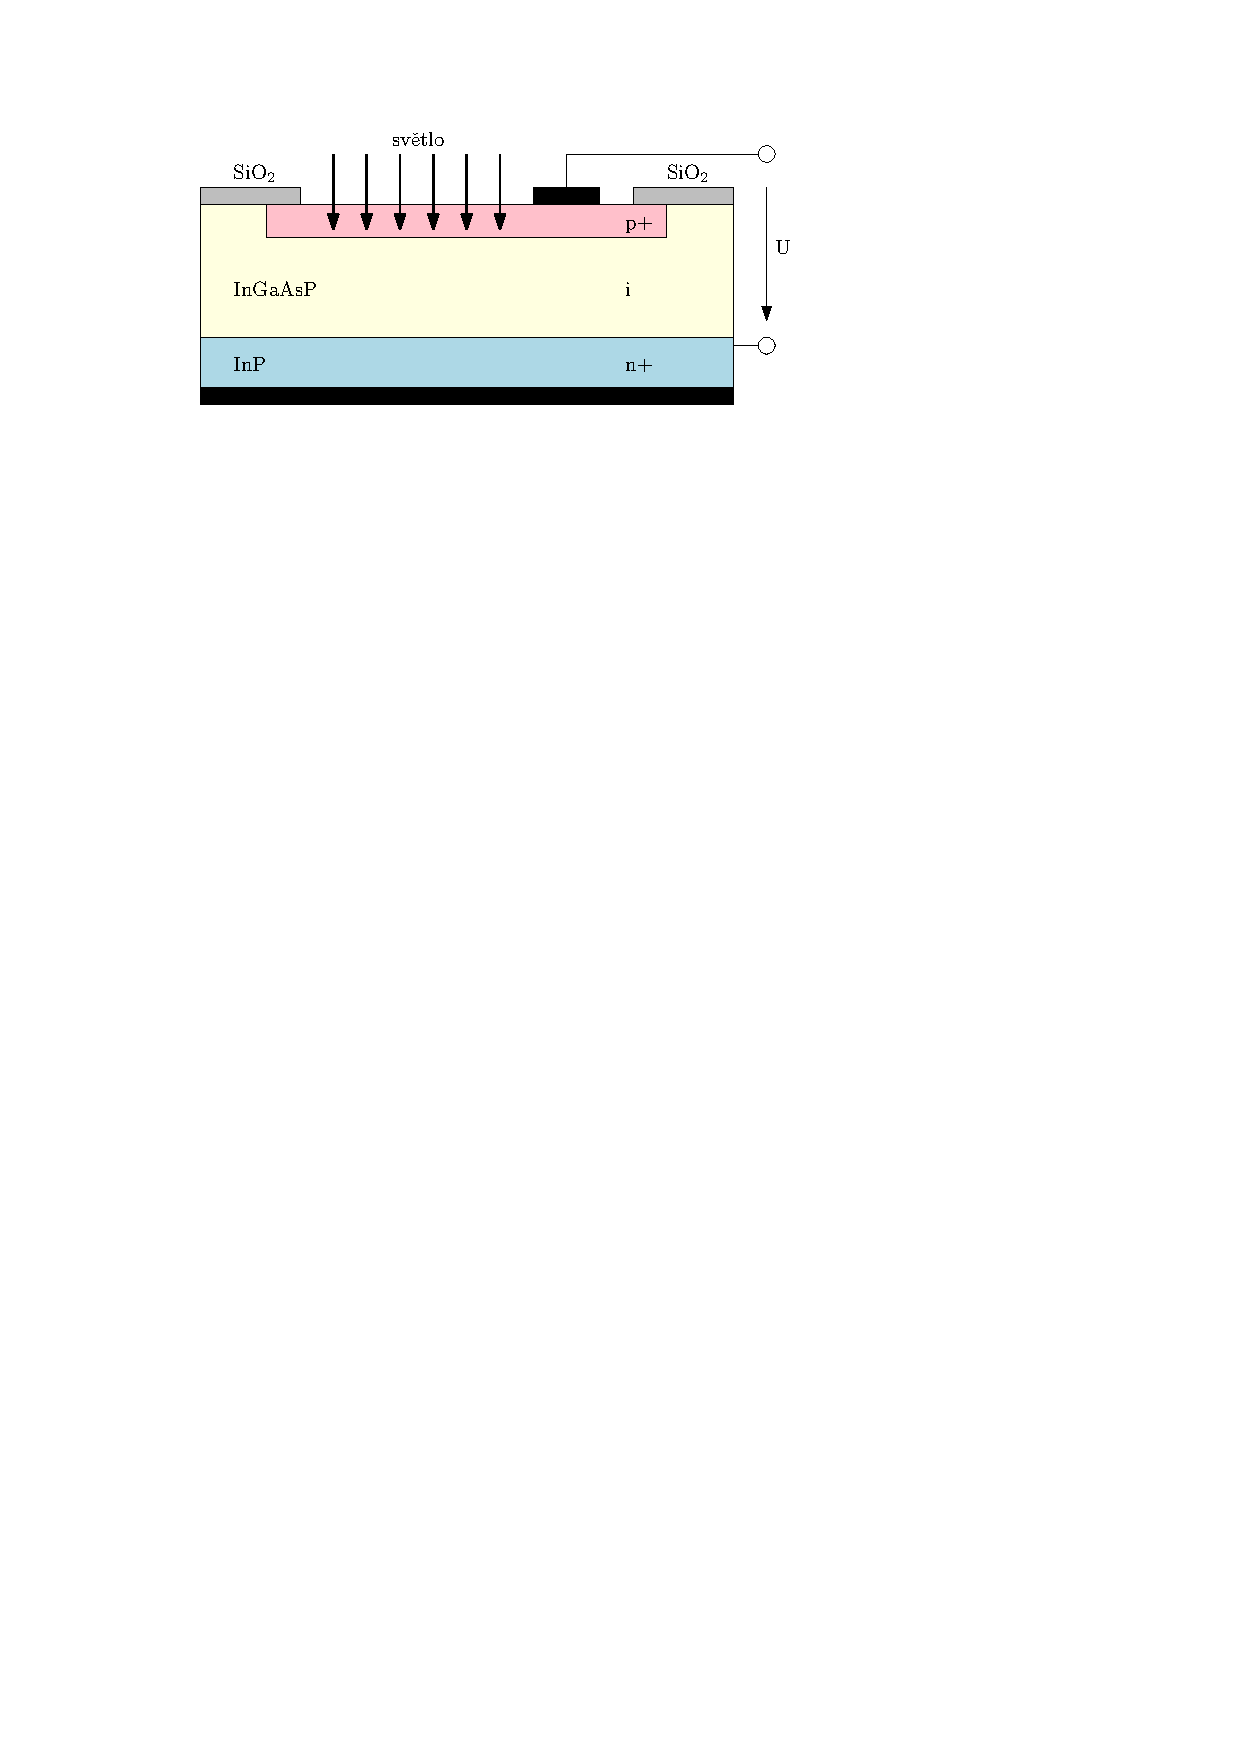
\includegraphics[scale=1]{img/pin}
    \end{center}
    \caption{Struktura PIN diody}
\end{figure}

\subsubsection{Fototranzistor}
Fototranzistor je fotodioda s tranzistorem jako zesilovačem fotonového proudu. Díky zesílení signálu je schopen detekovat i nižší intenzitu záření. Jeho nevýhodou je, že má $\beta$ větší parazitní kapacitu ($\beta$ je proudový zesilovací činitel), která omezuje jeho mezní frekvenci. Proto není vhodný pro měření rychlých signálů.

\begin{figure}[H]
    \begin{center}
        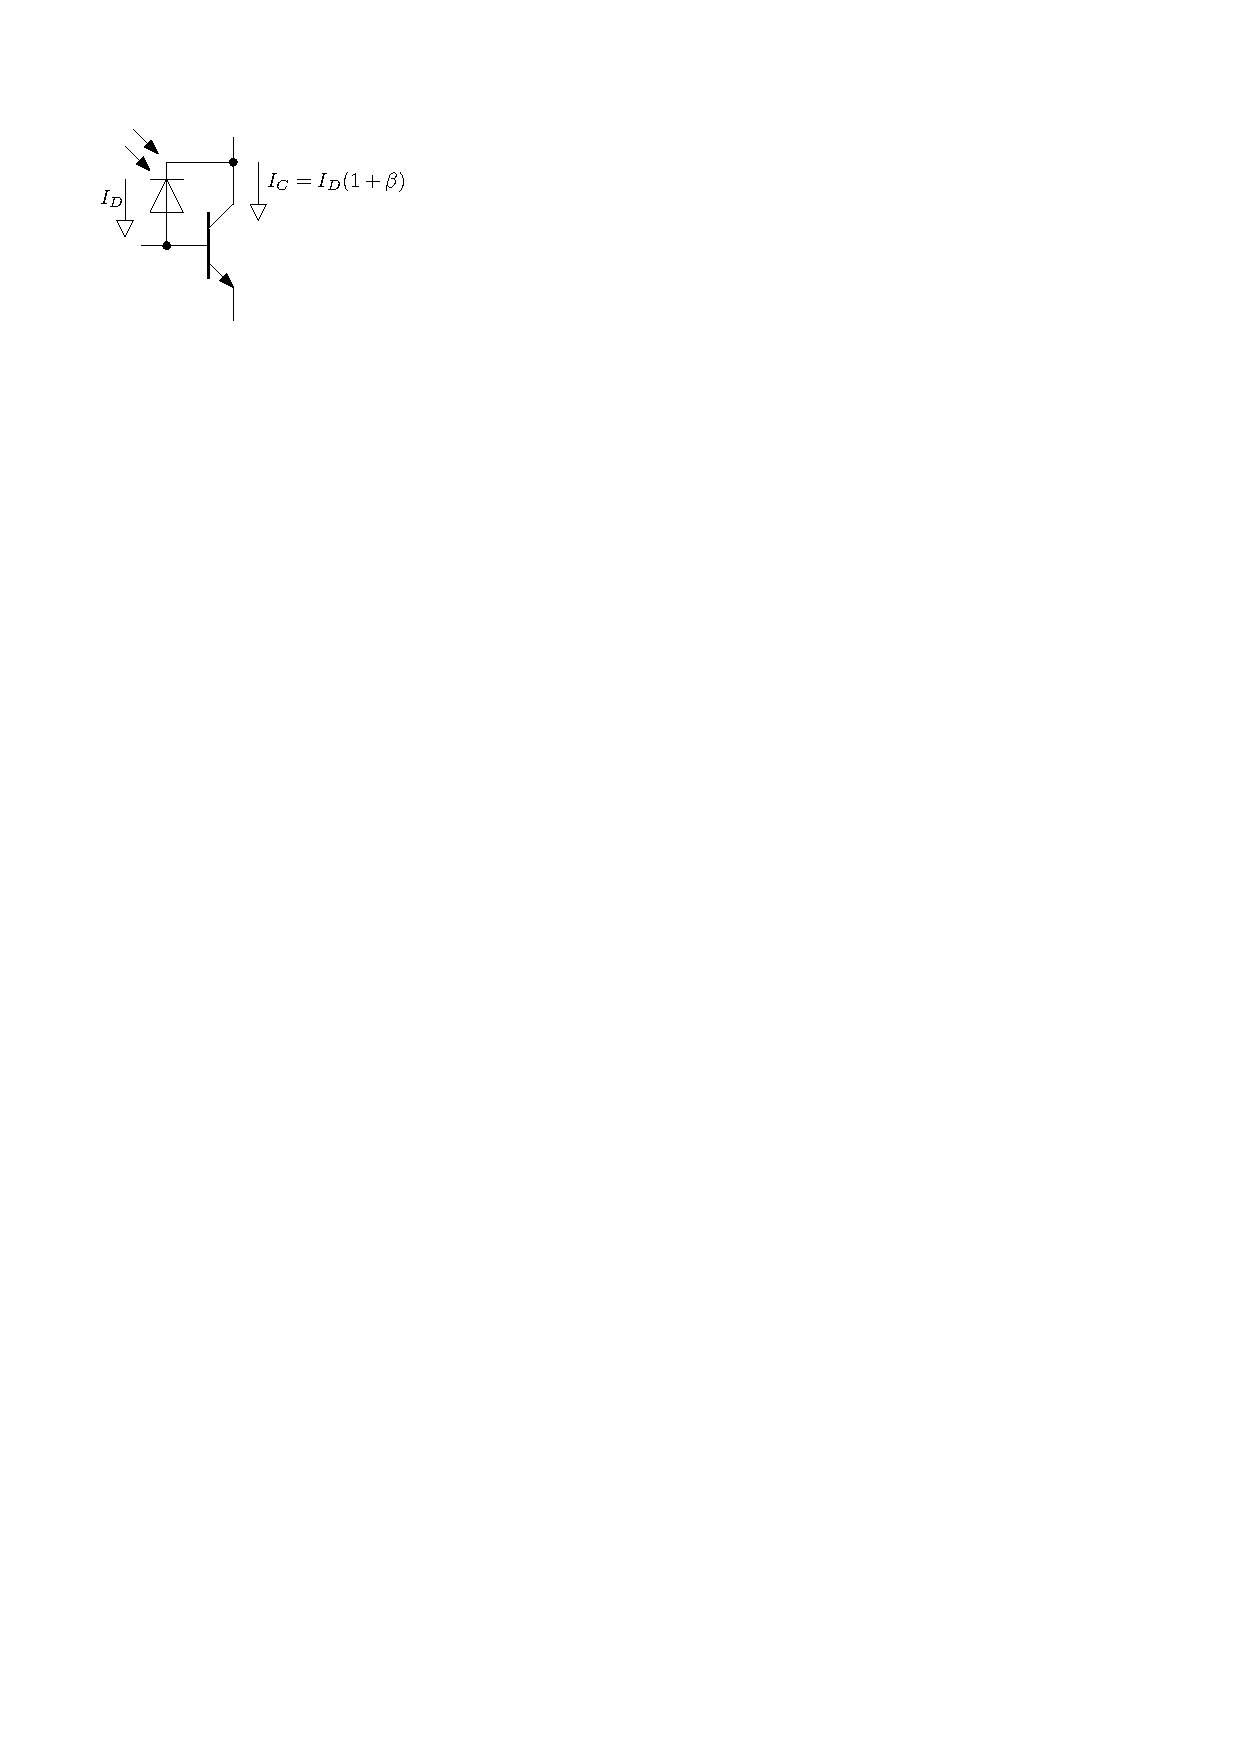
\includegraphics[scale=1]{img/foto-tran}
    \end{center}
    \caption{Náhradní schéma fototranzistoru}
\end{figure}

\subsubsection{Integrované přijímače}
Integrované optické přijímače mají na jednom čipu integrovanou kromě fotodiody i další elektroniku. Zpravidla obsahují vstupní zesilovač, pásmovou propust, demodulátor a výstupní zesilovač. Ještě je to třeba dopsat.

\begin{figure}[H]
    \begin{center}
        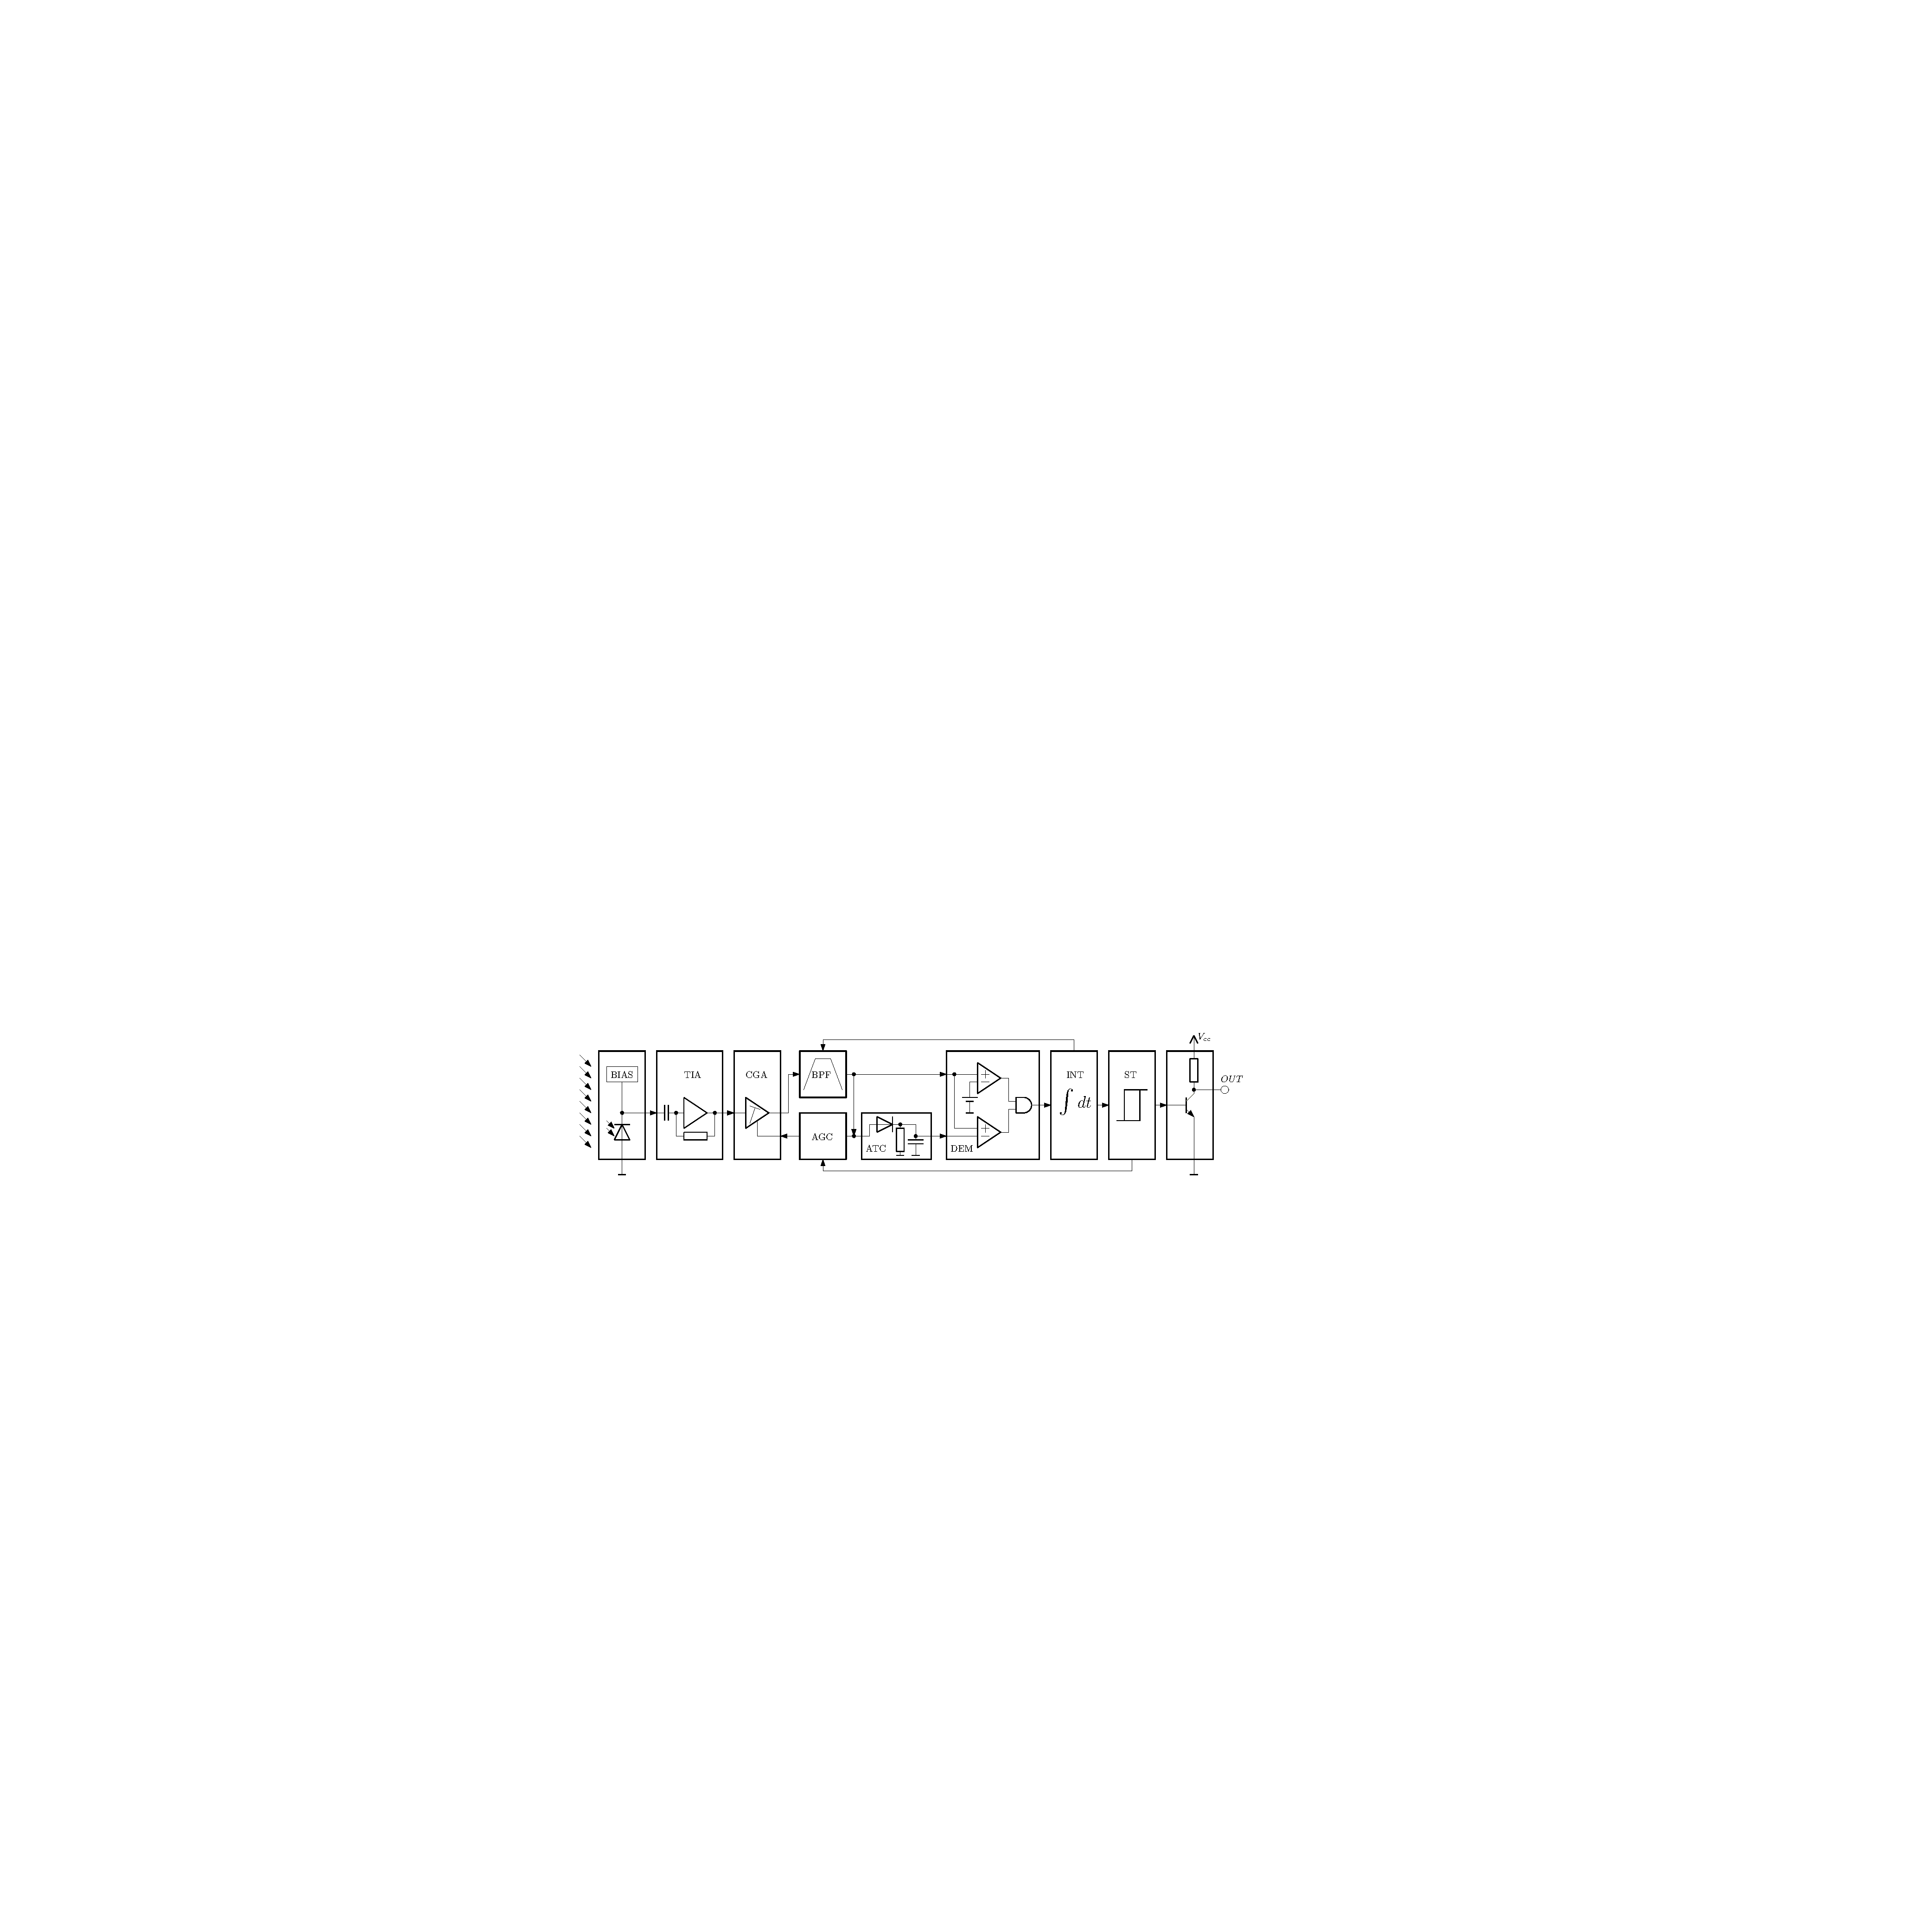
\includegraphics[width=\textwidth]{img/ir-rx}
    \end{center}
    \caption{Blokové schéma integrovaného přijímače OSRB38C9BA}
\end{figure}
